\documentclass{article}
% Change "article" to "report" to get rid of page number on title page
\usepackage{amsmath,amsfonts,amsthm,amssymb}
\usepackage{setspace}
\usepackage{Tabbing}
\usepackage{fancyhdr}
\usepackage{lastpage}
\usepackage{extramarks}
\usepackage{chngpage}
\usepackage{soul,color}
\usepackage{graphicx,float,wrapfig}
%\usepackage{listings}
\usepackage{float}
\usepackage{subfigure}
\usepackage{enumitem}
\usepackage{hyperref}
\usepackage{mathptmx}
%\usepackage{algpseudocode}

\newtheorem{definition}{Definition}
\newtheorem{remark}{Remark}
\newtheorem{theorem}{Theorem}
\newtheorem{lemma}[theorem]{Lemma}
\newtheorem{corollary}[theorem]{Corollary}
\newtheorem{fact}[theorem]{Fact}

% In case you need to adjust margins:
\topmargin=-0.45in      %
\evensidemargin=0in     %
\oddsidemargin=0in      %
\textwidth=6.5in        %
\textheight=9.0in       %
\headsep=0.25in         %
\onehalfspacing

\title{Bass IOR Syllabus: Programming Techniques and Algorithms for 3D Geometry}
\author{Instructor: Chris Tralie, ABD Topology/Applied Geometry, Duke University Department of Electrical Engineering}

\graphicspath{ {./COMPSCI299/} }

\begin{document}



\maketitle

Please visit \url{http://people.duke.edu/~cjt16/COMPSCI299} for an online version of this syllabus, which includes links to PDFs of most references

\section{Overview}
This hands on course will be a broad introduction to the world of 3D geometry, as seen by a computer. Students will learn how to efficiently represent, match, and morph 3D shapes through a series of programming assignments. Students will also gain an appreciation for many practical computational issues and tradeoffs in designing such algorithms. For engineering and computer science students, the course can serve as an accessible, visually-oriented introduction to more advanced mathematical topics in geometry, such as Riemannian manifolds, diffusion geometry, and symmetries. Conversely, it can serve as a practical applications course and an opportunity to develop important programming skills for math majors who are already familiar with such topics.  The course will culminate in a collaborative final project related to big data and 3D shapes, which will assist researchers in the Information at Duke (IID) program with unsolved, real-world problems.

\section{Textbooks}
There is no official textbook for the course, since it covers such a broad array of topics. Some of the original papers on the techniques that will be presented in the course are linked from the syllabus. If you would like to have a textbook, the two below are personal favorites of mine and would be the most useful references to go along with the course 

\begin{enumerate}

\item {\em Numerical Geometry of Nonrigid Shapes} by Alexander M. Bronstein, Michael M. Bronstein, and Ron Kimmel \cite{Bronstein2008}

\item {\em Mathematics for 3D Game Programming and Computer Graphics} by Eric Lengyel \cite{lengyel2012mathematics}

\end{enumerate}

\section{Prerequisites}
Undergraduate linear algebra, undergraduate algorithms, moderate programming experience (assignments will be written in Python).  Linear algebra will be reviewed at the beginning of the course, but algorithms and data structures is a hard prerequisite.

\section{Grading}
\begin{itemize}
\item Assignments: 60$\%$ (12$\%$ for each of 5)
\item Final Project: 40$\%$
\end{itemize}

\section{Policies}

\begin{itemize}
\item Each student has 7 late days available to be used on the assignments throughout the semester. Use them or lose them. They may be spread out over all the assignments or used all at once. You will indicate how many late days you have used on each assignment.

\item Once all late days have been used, you will lose points on the assignment at this rate

\begin{itemize}

\item    95$\%$ for work submitted up to 6 hours late
\item    90$\%$ for work submitted up to 12 hours late
\item    85$\%$ for work submitted up to 24 hours late
\item    75$\%$ for work submitted up to 48 hours late
\item    50$\%$ for work submitted up to 96 hours late
\item    0$\%$ for work submitted more than 96 hours late
\end{itemize}

\item {\em Cheating policy}: If you are found to have copied code from another student, or if you have used code from the web without asking me first, you will get a negative 100$\%$ on that assignment. Coding should be a fun, lifelong skill, so take the time to learn to do it on your own! And please ask for help if needed, rather than cheating. Note that a 50$\%$ on an assignment is far better than a negative 100$\%$, and it's likely you will get at least that if you try, so remember this if the temptation to cheat arises

\end{itemize}


\section{Syllabus}

Readings are provided for your reference where appropriate. I will try to spend 5 minutes at the end of each class to give you a birds eye view of the denser papers if you want to dive into them. Enjoy! 



\begin{tabular}{ | l | l | l | }
  \hline
  \large Lecture Number & \large Topic & \large References \\ \hline 
  \multicolumn{3}{l}{ } \\        
  \multicolumn{3}{l}{\Large Unit 1: Fundamentals} \\ \hline    
  	1. & Course Overview, Sneak Preview & \\ \hline
  	2. & Linear Algebra Review (Eigenvalues, Eigenvectors) & \\ \hline
  	3. & Geometric Primitives and Rigid Transformations & \cite{lengyel2012mathematics} Ch. 1-3 \\ \hline
  	4. & The Spatial Fourier Transform & \\ \hline

  \multicolumn{3}{l}{ } \\        
  \multicolumn{3}{l}{\Large Unit 2: Point Clouds and Shape Matching} \\ \hline 
    5. & Point Clouds Overview & \url{http://www.pointclouds.org} \\ \hline       
  	6. & Iterative Closest Points and Hausdorff Distance & \cite{chen1992object}, \cite{Bronstein2008} Ch. 6.2 \\ \hline
  	7. & 3D Shape Descriptors & \cite{ankerst19993d}, \cite{osada2002shape} \\ \hline
  	8. & Symmetries: Part 1 & \cite{thrun2005shape} \\ \hline
  	9. & Symmetries: Part 2 & \cite{kazhdan2004reflective}, \cite{podolak2006planar} \\ \hline
  	
  \multicolumn{3}{l}{ } \\        
  \multicolumn{3}{l}{\Large Unit 3: Manifold Surface Representations} \\ \hline 

  	10. & Polygon Meshes &  \cite{botsch2007geometric} Ch. 1-3 \\ \hline
  	11. & Intro To Topology, Euler Numbers & \cite{richeson2012euler} \\ \hline %Present connection to betti numbers at a high level, cite harish's writeup
  	12. & Parametric and Implicit Surfaces &  \\ \hline       	
  	13. & Subdivision Surfaces & \cite{zorin1999subdivision} Ch. 1-2 \\ \hline
  	14. & Splines & \\ \hline


  \multicolumn{3}{l}{ } \\        
  \multicolumn{3}{l}{\Large Unit 4: Nonrigid Geometry} \\ \hline 
    15. & Laplacian Meshes &  \cite{sorkine2006laplacian} \\ \hline       
  	16. & Laplace Beltrami Spectra + Functional Maps &  \cite{ovsjanikov2012functional}, \cite{Rustamov2013} \\ \hline
  	17. & Diffusion Maps + The Heat Kernel Signature & \cite{sun2009concise}, \cite{Mahmoudi2009} \\ \hline
  	18. & Geodesics and Fast Marching & \cite{kimmel1998computing}, \cite{Memoli2005}, \cite{Bronstein2008} Ch. 5\\ \hline
  	19. & Generalized Multidimensional Scaling & \cite{bronstein2006generalized}, \cite{Bronstein2008} Ch. 9 \\ \hline
  	20. & Mesh Segmentation & \\ \hline
  	
  \multicolumn{3}{l}{ } \\        
  \multicolumn{3}{l}{\Large Unit 5: Geometry for 3D Rendering} \\ \hline 
    21. & Projective Geometry &  \\ \hline       
  	22. & Clipping and Filling & \cite{sutherland1974reentrant}  \\ \hline
  	23. & Ray Tracing & \cite{lengyel2012mathematics} Ch. 5 \\ \hline
  	24. & Image Sources & \cite{rindel2000use} \\ \hline
	25. & Sound Propagation Modeling & \\ \hline
  	26. & Beam Tracing &  \cite{heckbert1984beam}, \cite{funkhouser1998beam}, \cite{overbeck2007real} \\ \hline	

  \multicolumn{3}{l}{ } \\        
  \multicolumn{3}{l}{\Large Unit 6: Miscellaneous Geometric Topics (Time Permitting)} \\ \hline 
    27. & Convex Hulls &  \\ \hline       
  	28. & Voronoi Diagrams &   \\ \hline
  	29. & Approximate Nearest Neighbor & \\ \hline
  	30. & KDTrees, BSPTrees, OctTrees &  \\ \hline
 
\end{tabular}

\section{Assignments}

\begin{itemize}
\item There will be one (very fun!) programming assignment for each of the first 5 units on the syllabus.  A portion of the grade for each programming assignment will be determined automatically by running batch tests on your submitted code, and comparing to the correct solutions. The tests will not be known ahead of time, but they will be published after everyone has submitted their assignments (following a model similar to \url{http://www.topcoder.com}). The student(s) with the fastest running correct implementation will be awarded a 15$\%$ bonus on the assignment. If ``correctness" is on a spectrum (as with the shape retrieval assignment), those with the highest accuracy will also get a bonus.

\item There will also be an ``art contest" for every submission. Students will get extra credit for any submission whatsoever into the art contest, but the winner (as determined by a panel of anonymous judges) will get the most extra credit.

\item Note that every effort will be made to eliminate the overhead of developing your applications.  I am a firm believer in the concept of ``skeleton code."  This means all of the mundane things like loading files, user interfaces, and rendering will be taken care of for you.  Your job will be to fill in the ``meat" of all of the algorithms.
\end{itemize}

The assignments are as follows

\begin{enumerate}
\item {\Large Geometric Primitives}: \normalsize You will develop code to do rotations, translations, scales, and intersections of primitive geometric objects, such as lines, planes, cones, and boxes.

\item {\Large Point Cloud Descriptors for Shape Retrieval}: \normalsize You will develop algorithms to classify point clouds into shape categories, and there will be a competition to see who can best classify an unknown set of point clouds

\item {\Large Mesh Processing}: \normalsize You will create code to store and manipulate 3D triangle meshes.  You will implement some basic mesh processing algorithms, such as local smoothing, subdivision, normal computation, and basic hole filling

\item {\Large Laplacian Mesh Editing}: \normalsize You will implement an algorithm that allows users to stretch polygon meshes in a smooth, graceful way, using sparse matrices

\item {\Large Image Sources for Acoustic Simulations}: \normalsize You will use the image sources algorithm to model all specular reflections in a virtual environment modeled by a polygonal mesh, to simulate how sound propagates through that mesh.  At the end you will be able to hear what music sounds like played on arbitrarily-placed boom box in many different types of environments (large cities, elliptical whisper chambers, high reverb rooms)

\end{enumerate} 


\section{Final Project}
Students will work in teams on a semester long project to use the tools they learn in this class to address unsolved, real world problems, and each team will be paired with a researcher in the Information Initiative at Duke (IID) who will be the point person for the respective project.  Possible problems (depending on IID participation and need) may include

\begin{itemize}

\item Segmenting or visualizing structures in large 3D brain data

\item Analyzing the shape of lemur teeth to help evolutionary anthropologists (see \cite{boyer2011algorithms})

\item Learning facial expressions from 3D range scans of faces, and simulating ``PIE-Invariant" (Pose/Illumination/Expression Invariant) faces

\item Virtual restoration of medieval statues in the Nasher Museum

\end{itemize}

(Note: I have either personally been involved in all of the above projects, or I have collaborated with people working on them.  They are all ongoing in IID)

\bibliographystyle{plain} %Formats bibliography
\bibliography{ctralie_Syllabus}

\begin{figure}[t]
	\centering
	\subfigure{
	  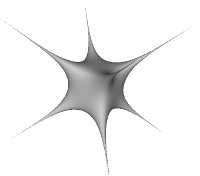
\includegraphics[width=0.3\textwidth]{cubemembrane2.png}
	}
	\subfigure{
	  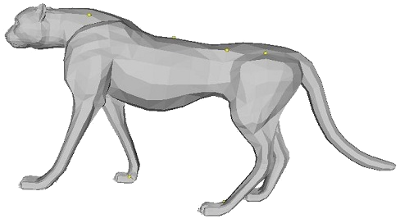
\includegraphics[width=0.4\textwidth]{deform.png}
	}
	\subfigure{
	  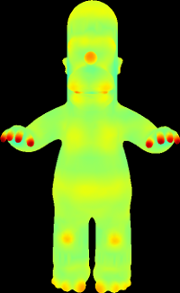
\includegraphics[width=0.2\textwidth]{HeatKernel.png}
	}
	\subfigure{
	  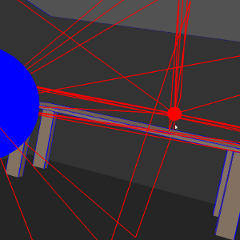
\includegraphics[width=0.28\textwidth]{imagesources.png}
	}
	\subfigure{
	  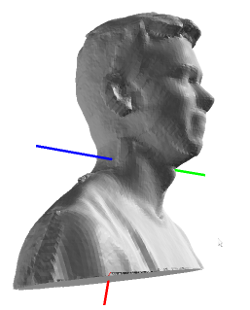
\includegraphics[width=0.25\textwidth]{pca.png}
	}
	\subfigure{
	  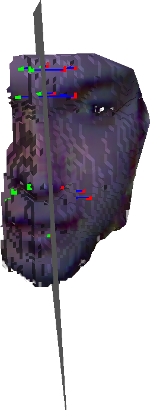
\includegraphics[width=0.2\textwidth]{prst.png}
	}	
	\subfigure{
	  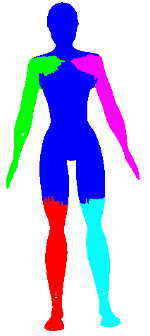
\includegraphics[width=0.15\textwidth]{segmentation.png}
	}	
\end{figure}

\end{document}
